\section{Overview of \FW{}}
\FW{} is developed to assist in performing source to target testing of pygrametl programs. Testing is performed at the system level, once an ETL has been put together. We illustrate this type of test in \ref{fig:sourcetotarget}. Here the ETL populates a DW using a set of sources. The DW is then tested, and test results are reported. In \FW{} the testing process evaluates a set of assertions that the tester makes about the resulting DW. Once testing is completed, \FW{} reports on each assertion, and whether it holds or not. Assertions are based upon the initial state of the system, which includes the contents of sources and DW before run. \FW{} can be used both to test new functionality and perform regression testing. Thus it is a tool useful both during before and after release. 

\begin{figure}
\centering
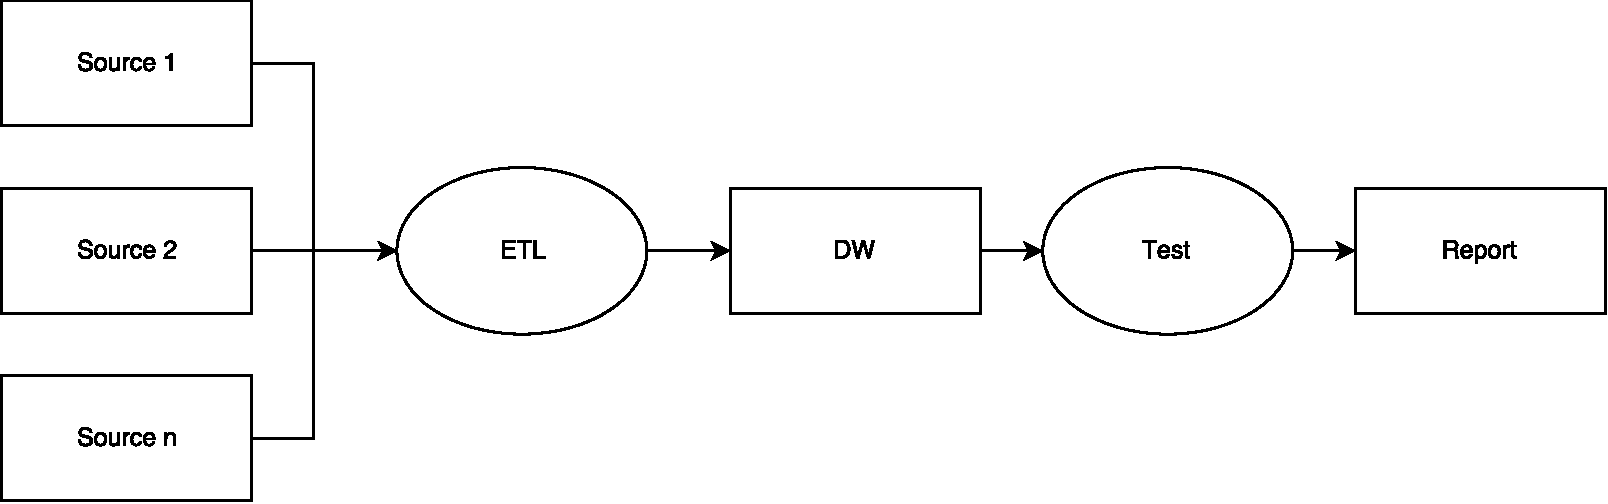
\includegraphics[width=0.5\textwidth]{figures/scenario.pdf}
\caption{Diagram of source to target test}
\label{fig:sourcetotarget}
\end{figure}

\subsection{Testing with \FW{}}
Exhaustive tests of a system are common. Rather to save resources, an adequate level of test coverage is defined. Test coverage describes requirements, which the system must live up to before testing is completed. From these requirements the tester can develop test cases, which ensure fulfillment of requirements. For \FW{} a test case is defined as an initial state of the system and a set of assertions. Thus \FW{} allows for testers to reach the level of test coverage agreed upon.

Often testers do not have access to actual data that their ETL will use once released. They are instead forced to define their own sources and DW  for their test cases. To avoid errors in the tests themselves, the test data needs to be small in size. This is acceptable as \FW{} does not focus upon  performance or stress testing. Some edge cases may also be absent from actual collected data. Thus even with access to actual data, testers may have issues with getting the needed test coverage. In \FW() a test data source can be given as a  PEP 249 connection or a list of dictionaries. A test DW can be given only through a PEP 249 connection. 

\subsection{Area of Test}
Assertions are central to \FW{}. However, in order to assist testers in making assertions, we must define, what has to be tested. Knowing what to test, we know what needs to be asserted. We choose \FW{} to assist in only data centered testing. Thus performance and security testing is ignored.  Even delimiting the scope of \FW{}, the litterature contains many different suggestions on what to test. We find the areas of Data Integrity, Data Loss and Business Rules to be of the greatest interest. These will be explained in the following: 

\subsubsection{Data Integrity}
For a DW to be useful we want there to be data integrity. That is, stored data is both accurate and consistent. 3 rules ensure data integrity:

\begin{itemize}
\item Entity integrity
\item Referential integrity
\item Domain integrity
\end{itemize}

Entity integrity concerns primary keys. It states that every table should have a primary key and that it should be unique and not null for each entry. Referential integrity is about foreign keys. It enforces that a foreign key should either refer to the primary key of another table or be null. This means that a foreign key can not refer to a primary key that does not exist. Domain integrity relates to the values taken on by attributes. It says that all attributes must have a defined domain. Likewise the values of attributes in all tuples should stay within their defined domain. Data integrity is important as it allows us to assert certain truths about our database. Such as each tuple in a table being identifiable or that a join between two tables is possible. Despite these advantages, DBMS' may not enforce them during loads. Loading data into a DW using an ETL usually involves a large amount of data and access to the DW is shut down temporarily. Checking each entry for data integrity can be expensive. Therefore a fast load often takes precedence over a safe load. If the ETL system is improperly designed, the DW ends up not having data integrity, which may hinder its usefulness. If the framework can assist in testing for data integrity, we can ensure future data integrity.

\subsubsection{Data Loss}
Through the ETL process, data from sources makes its way into a DW. This new data contains information relevant to future business analysis performed by users. However, information may get lost during the process. Data loss may occur in any of the three subprocesses. It is possible that the wrong data is extracted from the sources. Transformations may be faulty and produce an incorrect result. Loss during load may occur through truncation. Truncation occurs, when the datatype of a DW attribute cannot store the amount of data necessary. This often results in the data being cut to fit the data type, and thus data is lost. The result of any data loss is a DW not containing the needed information. This leads to poor business analysis. The framework should assist in ensuring that no data loss occurs during the process.

\subsubsection{Business Rules}
The term business rule is generally used for all rules applied to data stored in a database. This also includes data integrity as spoken about before. However data integrity could be seen as an ideal from which the business rules may differ. In the case of DWs the actual business rules often do not enforce entity integrity upon the fact table as the access of a specific entry may be unnecessary. Business rules however do not only pertain to data integrity as it is a rather broad term. An example of this could be an attribute relationships such as hierarchies. Another type of business rule could describe the schema of a specific table.


%% Vi har brug for noget text om at pygrametl presser os til at være generiske. PEP249. 
%% Skal kunne connecte vores tanker om assertions her til predicates længere fremme. 






